\chapter{Présentation de Wireshark}
\begin{onehalfspace}




\section{Présentation de l'outil}

\textbf{Wireshark} est un programme qui permet d'écouter ce qui passe sur le réseau. Concrètement, Wireshark récupère les paquets réseau qui arrivent sur l'interface réseau et interprète leur contenu intelligemment pour les présenter de façon intuitive. Il permet ainsi de voir tous les paquets à destination de la carte réseau. C'est ce que l'on appelle un \textbf{Sniffer}.


\section{Présentation de la fenêtre}

La fenêtre se compose en gros de quatre parties :
\begin{itemize}
\item les menus et commandes;
\item la présentation résumée des paquets reçus;
\item la présentation détaillée d'un paquet ciblé;
\item le contenu hexadécimal du paquet.
\end{itemize}


Le menu présenté en figure suivante est essentiellement composé des actions que nous pouvons faire avec Wireshark.

\begin{figure}[H]
\centering
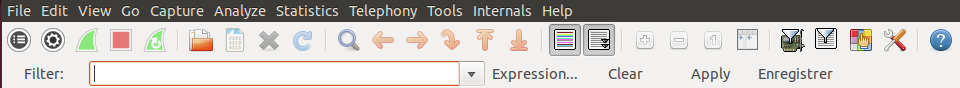
\includegraphics [width=160mm]{chapitre1/menu.png}
\caption{Menu de Wireshark}
\label{fig:menu}
\end{figure}


\vspace{1\baselineskip}


On peut voir en figure suivante la liste résumée des paquets reçus avec les adresses IP source et destination, le dernier protocole encapsulé ainsi que quelques informations sur le contenu du paquet.

\begin{figure}[H]
\centering
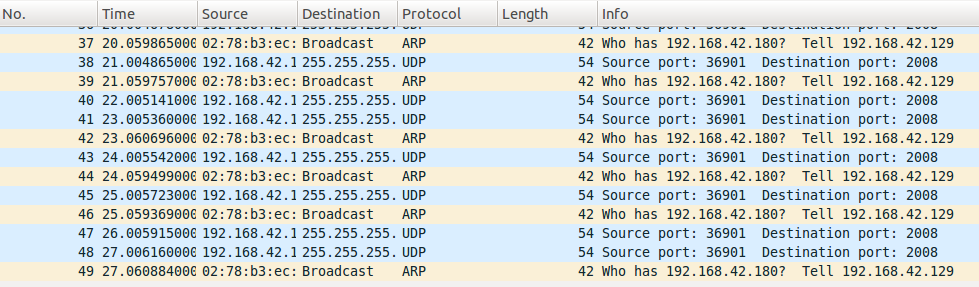
\includegraphics [width=190mm]{chapitre1/paquets.png}
\caption{La liste des paquets}
\label{fig:}
\end{figure}


\end{onehalfspace}
